\section{Prototype Implementation}
\label{sec:implementation}


This section should provide brief details of how the prototype has been implemented.
You may want to use come code snippets here, but only focus on core features and aspects.
You are not meant to copy/paste your whole application code into the report.
Focus for instance how other developers may run your application and how they might develop it further...


The example below shows how you may include code. There are similar
styles for many other langages - in case you do not use Java in your
project. You can wrap the listing into a figure in case you need to
refer to it. How to create a figure was shown in Section~\ref{sec:technology}.

\lstinputlisting[language=java]{code/BoksVolum.java}

\subsection{Backend}

We will now look into how the Kotlin code is organized. We use Kotlin with Spring Boot as the backend. The code is organized into three main services: EventService, PollService, and UserService. These handle the business logic. We also have class JwtService,  which provides token management for authentication.
 
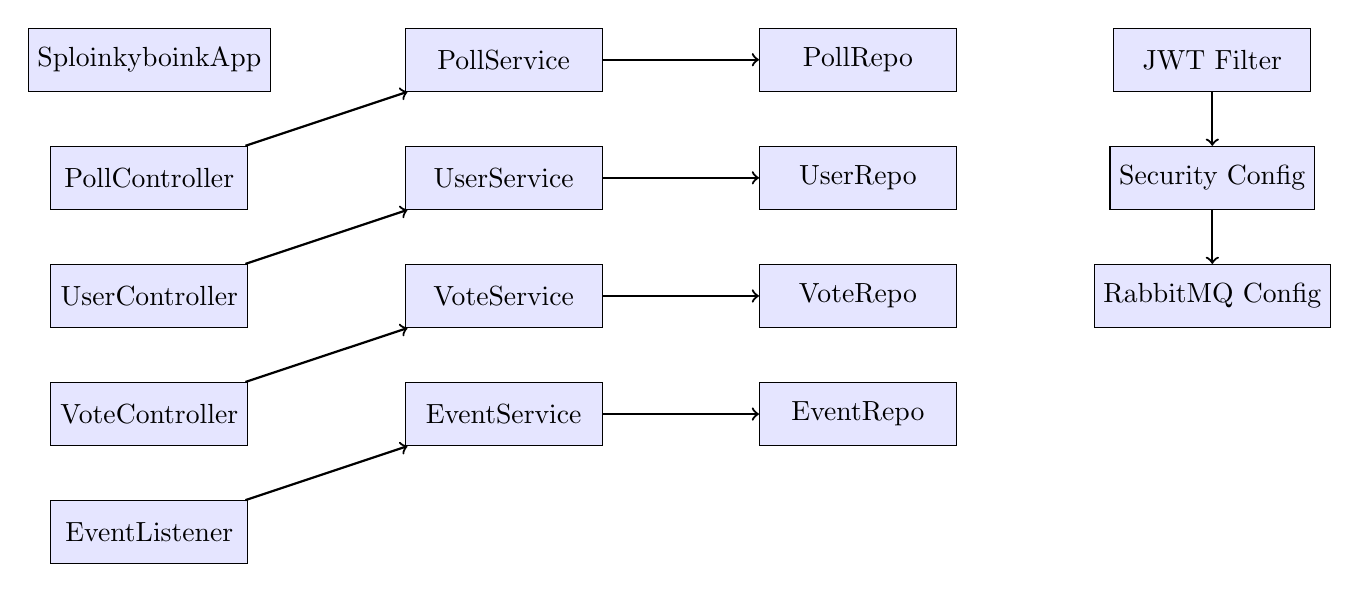
\begin{tikzpicture}[node distance=1.5cm]

% Define UML class styles
\tikzstyle{class} = [rectangle, draw=black, fill=blue!10, text centered, minimum height=0.8cm, minimum width=2.5cm]
\tikzstyle{arrow} = [->, thick, draw=black]

% Define nodes (classes)
\node[class] (sploinkyboinkApplication) {SploinkyboinkApp};
\node[class, below of=sploinkyboinkApplication] (pollController) {PollController};
\node[class, below of=pollController] (userController) {UserController};
\node[class, below of=userController] (voteController) {VoteController};
\node[class, below of=voteController] (eventListener) {EventListener};

% Define second layer nodes (Services)
\node[class, right of=sploinkyboinkApplication, xshift=3cm] (pollService) {PollService};
\node[class, below of=pollService] (userService) {UserService};
\node[class, below of=userService] (voteService) {VoteService};
\node[class, below of=voteService] (eventService) {EventService};

% Define third layer nodes (Repositories)
\node[class, right of=pollService, xshift=3cm] (pollRepository) {PollRepo};
\node[class, below of=pollRepository] (userRepository) {UserRepo};
\node[class, below of=userRepository] (voteRepository) {VoteRepo};
\node[class, below of=voteRepository] (eventRepository) {EventRepo};

% Define fourth layer nodes (Security)
\node[class, right of=pollRepository, xshift=3cm] (jwtAuthFilter) {JWT Filter};
\node[class, below of=jwtAuthFilter] (securityConfig) {Security Config};

% Define fifth layer nodes (Configurations)
\node[class, below of=securityConfig] (rabbitMQConfig) {RabbitMQ Config};

% Relationships (arrows)
\draw[arrow] (pollController) -- (pollService);
\draw[arrow] (userController) -- (userService);
\draw[arrow] (voteController) -- (voteService);
\draw[arrow] (eventListener) -- (eventService);

\draw[arrow] (pollService) -- (pollRepository);
\draw[arrow] (userService) -- (userRepository);
\draw[arrow] (voteService) -- (voteRepository);
\draw[arrow] (eventService) -- (eventRepository);

\draw[arrow] (jwtAuthFilter) -- (securityConfig);
\draw[arrow] (securityConfig) -- (rabbitMQConfig);

\end{tikzpicture}

\vspace{1cm}

% External explanations
\noindent
\textbf{SploinkyboinkApp:} The main application class for the Sploinkyboink application.\\
\textbf{PollController, UserController, VoteController, EventListener:} Classes that handle HTTP requests related to polls, users, votes, and events, respectively.\\
\textbf{PollService, UserService, VoteService, EventService:} Business logic classes for polls, users, votes, and events.\\
\textbf{PollRepo, UserRepo, VoteRepo, EventRepo:} Data access classes for interacting with the database for polls, users, votes, and events.\\
\textbf{JWT Filter:} Filters HTTP requests for JWT authentication.\\
\textbf{Security Config:} Configures security settings and authentication for the application.\\
\textbf{RabbitMQ Config:} Configures RabbitMQ for message processing.


Here is a high-level overview of what each service does:
\begin{itemize}
    \item \textbf{EventService:}
    \begin{itemize}
        \item \textbf{Logging Events:} This service is responsible for logging various events related to polls and votes. It saves events to a database and sends messages to a RabbitMQ queue.
        \item \textbf{Event Types:} It handles specific types of events such as:
        \begin{itemize}	
            \item \textbf{VoteEvent:} When a user votes on a poll.
            \item \textbf{PollCreated:} When a new poll is created.
            \item \textbf{PollEdited:} When an existing poll is edited.
        \end{itemize}
        The events include details such as the poll ID, the question, options, and timestamp.
    \end{itemize}

    \item \textbf{PollService:}
    \begin{itemize}
        \item \textbf{Poll Management:} This service manages the lifecycle of polls, including creating, retrieving, editing, and deleting polls.
        \item \textbf{Voting Logic:} It also manages voting on polls, ensuring that users can only vote once, that polls are active, and allowing users to edit or delete their votes.
        \item \textbf{Results Calculation:} It calculates and retrieves the results of the polls based on the votes received.
    \end{itemize}

    \item \textbf{UserService:}
    \begin{itemize}
        \item \textbf{User Management:} This service handles user registration, authentication, and management. It ensures that users' usernames and emails are unique and validates passwords against defined criteria.
        \item \textbf{CRUD Operations:} It provides functionality to create, read, update, and delete user information.
    \end{itemize}

    \item \textbf{Achievements of the Code:}
    \begin{itemize}
        \item \textbf{Polling Functionality:} The application allows users to create, manage, and participate in polls, capturing user votes and managing their options.
        \item \textbf{Event Tracking:} It tracks important actions within the application, such as when polls are created or edited, and when votes are cast, providing a basis for auditing or analytics.
        \item \textbf{User Management:} It provides security by validation of users.
        \item \textbf{Integration with Messaging:} By integrating RabbitMQ, it supports event-driven architecture, allowing for scalability and decoupling of services.
    \end{itemize}
\end{itemize}

